\documentclass[conference]{IEEEtran}
\IEEEoverridecommandlockouts

\usepackage[utf8]{inputenc}
\usepackage{amsmath,amssymb,amsfonts}
\usepackage{algorithmic}
\usepackage{algorithm}
\usepackage{graphicx}
\usepackage{booktabs}
\usepackage{multirow}
\usepackage[caption=false,font=footnotesize]{subfig}
\usepackage{xcolor}
\usepackage{cite}
\usepackage{url}
\usepackage{bm}

\graphicspath{{figures/}}

% ============================================================
\title{Semantic Digital Twins and Multi-Agent Reinforcement Learning for IoT Resource Allocation}
% ============================================================

\author{
\IEEEauthorblockN{Nguyen Thi Huyen Trang$^{1}$,
Hoang Trong Binh$^{2}$,
Nguyen Quoc Khanh$^{2}$,
Ngo Van Khuong$^{3}$,
Pham Van Tiep$^{3}$,
Dinh Van Linh$^{3,\dagger}$}

\IEEEauthorblockA{$^{1}$Le Quy Don Technical University, Hanoi, Vietnam\\ Email: trangcucheng@gmail.com}
\IEEEauthorblockA{$^{2}$Institute of Information and Communication Technology, Le Quy Don Technical University, Hanoi, Vietnam\\ Email: binhht99@lqdtu.edu.vn, khanhbk29@gmail.com}
\IEEEauthorblockA{$^{3}$Academy of Cryptography Techniques, Hanoi, Vietnam\\ Email: Khuogn2005@gmail.com, ptiep94@gmail.com, \texttt{vanlinh@actvn.edu.vn}}
\IEEEauthorblockA{$^{\dagger}$Corresponding author: \texttt{vanlinh@actvn.edu.vn}}
}

\begin{document}
\maketitle

% ============================================================
\begin{abstract}
% ============================================================
Effective IoT network management requires simultaneous semantic feature
compression, real-time channel quality monitoring, anomaly detection, and
adaptive resource allocation. Existing approaches address these tasks in
isolation, lacking a unified system that jointly exploits temporal dynamics
and multi-agent coordination. A three-stage framework is proposed combining:
(i) a Variational Autoencoder (VAE) for semantic compression of raw IoT
features into compact latent representations; (ii) an Extended Kalman Filter
(EKF)-based Digital Twin for joint connection quality classification and
anomaly detection via the Normalized Innovation Squared (NIS) test; and
(iii) Multi-Agent Deep Reinforcement Learning with Graph Attention Networks
(MADRL-GAT) for cooperative resource allocation guided by semantic state
and quality feedback. Experiments on three real-world IoT datasets---Sigfox
Antwerp (14,377 samples), LoRaWAN Italy (190,502 samples), and Indoor WiFi
(1,100 samples)---demonstrate that the proposed Digital Twin component achieves
quality classification AUC up to 0.972, outperforming K-Means by up to
80.4\% on LoRaWAN, while attaining anomaly detection AUC up to 0.987 on
the Indoor dataset. The MADRL-GAT module converges stably within 50
episodes, yielding evaluation rewards of 1,916, 2,519, and 3,089
respectively.
\end{abstract}

\begin{IEEEkeywords}
Internet of Things, semantic communications, variational autoencoder,
digital twin, Extended Kalman Filter, multi-agent reinforcement learning,
graph attention network, anomaly detection, resource allocation
\end{IEEEkeywords}

% ============================================================
\section{Introduction}
\label{sec:intro}
% ============================================================

\IEEEPARstart{T}{he} explosive growth of IoT deployments---spanning smart
cities, industrial sensing, and indoor positioning---has introduced
unprecedented demands on wireless network infrastructure. Devices operating
across heterogeneous technologies (Sigfox, LoRaWAN, WiFi) continuously
generate high-dimensional telemetry streams that must be processed, monitored,
and acted upon with minimal latency and energy overhead~\cite{ref_iot_survey}.
Two fundamental challenges arise: the raw feature space is high-dimensional
and noisy, making downstream learning inefficient; and the network state
evolves continuously in time, requiring adaptive mechanisms that simultaneously
classify connection quality and detect anomalous behaviour.

\textbf{Semantic compression for wireless networks.}
Liu et al.~\cite{ref_vae_wireless} proposed a task-adaptive semantic
compression scheme employing a VAE to encode raw sensor observations into
compact, task-relevant representations, substantially reducing communication
overhead in resource-constrained networks. The compression rate adapts to
instantaneous channel quality, yielding strong reconstruction fidelity across
diverse wireless conditions. However, the scheme targets static point-to-point
links without temporal state tracking, provides no anomaly-detection
capability, and does not coordinate multiple agents---restricting applicability
to the dynamic, heterogeneous IoT settings considered in this work.

\textbf{Deep reinforcement learning for IoT resource allocation.}
Hazarika et al.~\cite{ref_marl_wireless} developed a deep RL framework for
computation offloading in Internet-of-Vehicles (IoV) networks, training DQN
agents on raw network-state features to achieve adaptive resource management
under time-varying interference. The approach demonstrates competitive
performance with low control overhead. A key limitation is that raw,
high-dimensional feature vectors serve as the agent state without semantic
compression, inflating the effective state space and degrading sample
efficiency; moreover, no channel-quality feedback enters the reward signal,
preventing the agent from distinguishing nominal from degraded link conditions.

\textbf{Digital twin-assisted resource management.}
Hazarika et al.~\cite{ref_dt_uav} integrated a digital twin with a hybrid
machine learning classifier for resource allocation in UAV-aided IoV networks.
The digital twin enables one-step-ahead channel prediction, yielding
measurable gains over purely reactive baselines. Nevertheless, quality
classification employs fixed decision thresholds that cannot adapt to
heterogeneous dataset statistics, anomaly detection is absent, and raw
features are fed directly to the allocation module without semantic
compression---leaving the system unable to flag silent sensor faults or
generalize across heterogeneous channel conditions.

\textbf{Semantic digital twins for multi-agent coordination.}
Most closely related to the present work, Hazarika et al.~\cite{ref_semadt}
combined semantic compression, predictive digital twin forecasting, and
multi-agent deep RL with a graph neural network (GNN) for maritime
search-and-rescue IoT operations, demonstrating that semantic state inputs
and DT-predicted quality signals together substantially outperform
non-predictive MARL baselines. Despite this advance, the GCN layer applies
symmetric neighborhood aggregation, whereas graph attention
networks~\cite{ref_gat_comm} better capture heterogeneous inter-agent
relationship strengths via learned attention weights. Furthermore, the anomaly
detector relies on a fixed scalar threshold rather than a statistically
principled multivariate test~\cite{ref_anomaly_survey,ref_lof}, and
validation is confined to a single maritime domain, leaving generalization
across heterogeneous IoT technologies unexplored.

\textbf{Contributions.} Three persistent gaps are identified: (1) semantic
compression, channel monitoring, and resource allocation are treated as
independent modules; (2) existing digital twin implementations perform either
quality classification \emph{or} anomaly detection, but not both within a
single principled state estimator; (3) no prior system has been validated
across heterogeneous IoT technologies in a unified architecture. This paper
addresses all three gaps:
\begin{itemize}
\item \textbf{Unified three-stage framework.} A three-stage framework coupling
VAE semantic compression, EKF Digital Twin monitoring, and MADRL-GAT resource
allocation is proposed. Compressed latent codes serve as both the MADRL state
space and input for quality-aware reward computation.
\item \textbf{Joint quality classification and anomaly detection.}
The EKF Digital Twin classifies connection quality via a data-adaptive
Youden's J threshold on estimated RSSI, and flags anomalies via the NIS
chi-squared test---both within a single filter pass.
\item \textbf{Multi-technology evaluation.} Validation is performed on three
real-world datasets spanning Sigfox, LoRaWAN, and WiFi IoT technologies,
demonstrating robustness across heterogeneous channel conditions.
\end{itemize}

The remainder of this paper is organised as follows. Section~\ref{sec:model}
presents the system model. Section~\ref{sec:problem} formulates the
optimization problem. Section~\ref{sec:method} details the proposed
framework. Section~\ref{sec:experiments} reports experimental results.
Section~\ref{sec:conclusion} concludes the paper.

% ============================================================
\section{System Model}
\label{sec:model}
% ============================================================

\subsection{IoT Network Model}

Consider a heterogeneous IoT network comprising $N$ nodes indexed by
$i\in\{1,\ldots,N\}$, where each node periodically transmits sensor
readings over a wireless channel to a gateway or base station. Let
$\mathbf{x}_i(t)\in\mathbb{R}^d$ denote the raw feature vector
observed by node $i$ at time $t$, comprising signal strength measurements
and sensor readings (e.g., RSSI per base station, SNR, temperature,
humidity, battery level).

\subsection{Channel State and Quality Model}

The quality of the wireless link for node $i$ is characterized by two
key indicators: the mean received signal strength ${\rm RSSI}_i(t)$
and the number of active base stations $n^{\rm BS}_i(t)$. The
two-dimensional channel state vector is defined as
\begin{equation}
\mathbf{s}_i(t) = \bigl[{\rm RSSI}_i(t),\; n^{\rm BS}_i(t)\bigr]^\top
\in \mathbb{R}^2.
\label{eq:channel_state}
\end{equation}
A connection is classified as \emph{good quality} if
${\rm RSSI}_i(t) \geq \tau_i$, where $\tau_i$ is a dataset-adaptive
threshold. Due to severe class imbalance in practical deployments
(e.g., only 1.9\% good-quality samples in the Sigfox Antwerp dataset),
$\tau_i$ is set to the median RSSI to yield balanced binary labels.

\subsection{Resource Allocation and Communication Model}

At each decision epoch, node $i$ selects a discrete action
$a_i(t)\in\{1,\ldots,A\}$ representing its resource configuration
(e.g., transmission power level, spreading factor, or channel index).
Let $h_{i,0}(t)$ denote the complex channel gain between node $i$ and
its designated base station at time $t$, incorporating both large-scale
path-loss and small-scale fading. The received
signal-to-interference-plus-noise ratio (SINR) $\gamma_i(t)$ is:
\begin{equation}
\gamma_i(t) = \frac{P_i(t) |h_{i,0}(t)|^2}{\displaystyle\sum_{j \neq i} P_j(t) |h_{j,0}(t)|^2 + \sigma_n^2},
\label{eq:sinr_v0}
\end{equation}
where $P_i(t)$ is the transmission power associated with action $a_i(t)$,
$\sum_{j \neq i} P_j(t)|h_{j,0}(t)|^2$ is the co-channel interference from
concurrent transmissions, and $\sigma_n^2$ is the AWGN power. The achievable
rate $R_i(t)=B\log_2(1+\gamma_i(t))$ enters the network utility in
Section~\ref{sec:problem}. Nodes are connected through a graph
$\mathcal{G}=(\mathcal{V},\mathcal{E},\mathbf{A})$, where the adjacency
matrix $\mathbf{A}$ encodes inter-node proximity (spatial distance for
Sigfox, feature correlation for LoRaWAN, fully-connected for Indoor).

\subsection{Fault Model}

To evaluate anomaly detection in the absence of naturally labeled faults,
synthetic anomalies are injected into 5\% of each time-ordered sequence
via three fault types:
\begin{equation}
{\rm RSSI}_i^{\rm fault}(t) =
\begin{cases}
\mu_{\rm RSSI} + 2\sigma_{\rm RSSI} & \text{(Spike: interference)},\\
\mu_{\rm RSSI} - 2\sigma_{\rm RSSI} & \text{(Drop: attenuation)},\\
\mu_{\rm RSSI} + 1.5\sigma_{\rm RSSI} & \text{(Stuck: sensor drift)},
\end{cases}
\label{eq:fault}
\end{equation}
where Drop and Stuck additionally set $n^{\rm BS}_i=0$ to simulate
connectivity loss. Fault magnitudes are deliberately set within
$\pm2\sigma$ of the global RSSI distribution to avoid trivially detectable
statistical outliers.

% ============================================================
\section{Problem Formulation}
\label{sec:problem}
% ============================================================

The global objective is to optimize the framework across multiple decision
stages. The network-wide utility at time $t$ is:
\begin{equation}
U(t) = \sum_{i=1}^{N}\bigl[
  \hat{q}_i(t)\cdot R_i(t) - \lambda\, a_i(t)
  + \mu\,\mathbb{1}\!\bigl[\xi_i(t) < \chi^2_{0.95}(2)\bigr]
\bigr],
\label{eq:utility}
\end{equation}
where $\hat{q}_i(t)\in\{0,1\}$ is the Digital Twin quality label,
$\xi_i(t)$ is the NIS anomaly score, and $\lambda,\mu>0$ are weighting
coefficients. Solving simultaneously for the VAE parameters $(\phi,\theta)$
and the multi-agent actions $\{a_i\}$ in a single joint pass is
computationally intractable and prone to gradient instability. The
problem $(\mathcal{P})$ is therefore decomposed into a
\textit{sequential optimization paradigm} executed in two discrete phases,
aligned with the decoupled workflow illustrated in Fig.~\ref{fig:framework}.
In Phase~1, the semantic feature space is optimized offline to maximize
the evidence lower bound:
\begin{equation}
\phi^*, \theta^* = \arg\max_{\phi,\theta}\;\mathcal{L}_{\rm VAE}(\phi,\theta;\mathbf{X}),
\label{eq:vae_opt}
\end{equation}
subject to the reconstruction error bound. The optimized VAE encoder is
then frozen, and the deterministic latent representations
$\hat{\mathbf{z}}_i(t)=\bm{\mu}_{\phi^*}(\mathbf{x}_i(t))$ are propagated
downstream to minimize the state-space dimensionality. In Phase~2,
conditioned on these frozen semantic states, the decentralized RL
optimization problem $(\mathcal{P}_{\rm RL})$ is formulated as:
\begin{equation}
(\mathcal{P}_{\rm RL})\!:\;\max_{\{a_i\}}\; \mathbb{E}\!\left[\sum_{t=0}^{T}\sum_{i=1}^{N} U(t) \;\Bigg|\; \hat{\mathbf{z}}_i(t)=\bm{\mu}_{\phi^*}(\mathbf{x}_i(t))\right]
\label{eq:rl_opt}
\end{equation}
subject to:
\begin{align}
&\text{(C.2)}\;\; \hat{q}_i(t) = \mathbf{1}\!\bigl[\widehat{\rm RSSI}_{i,t}\geq\tau^*\bigr], \;\forall\, i,t,\label{c2}\\
&\text{(C.3)}\;\; \Pr\!\bigl[\xi_i(t)>\chi^2_{0.95}(2)\big|\text{normal}\bigr] \leq 0.05,\;\forall\, i,t,\label{c3}\\
&\text{(C.4)}\;\; a_i(t)\in\{1,\ldots,A\},\;\forall\, i,t.\label{c4}
\end{align}
Constraint~\eqref{c2} defines quality labels from the EKF-estimated RSSI
via Youden's J threshold $\tau^*$; \eqref{c3} controls the NIS false-alarm
rate; \eqref{c4} restricts actions to the discrete resource set. This
decoupled hierarchical formulation guarantees convergence and practical
feasibility, as detailed in the three-stage framework below.

% ============================================================
\section{Proposed Framework}
\label{sec:method}
% ============================================================

\begin{figure*}[t]
  \centering
  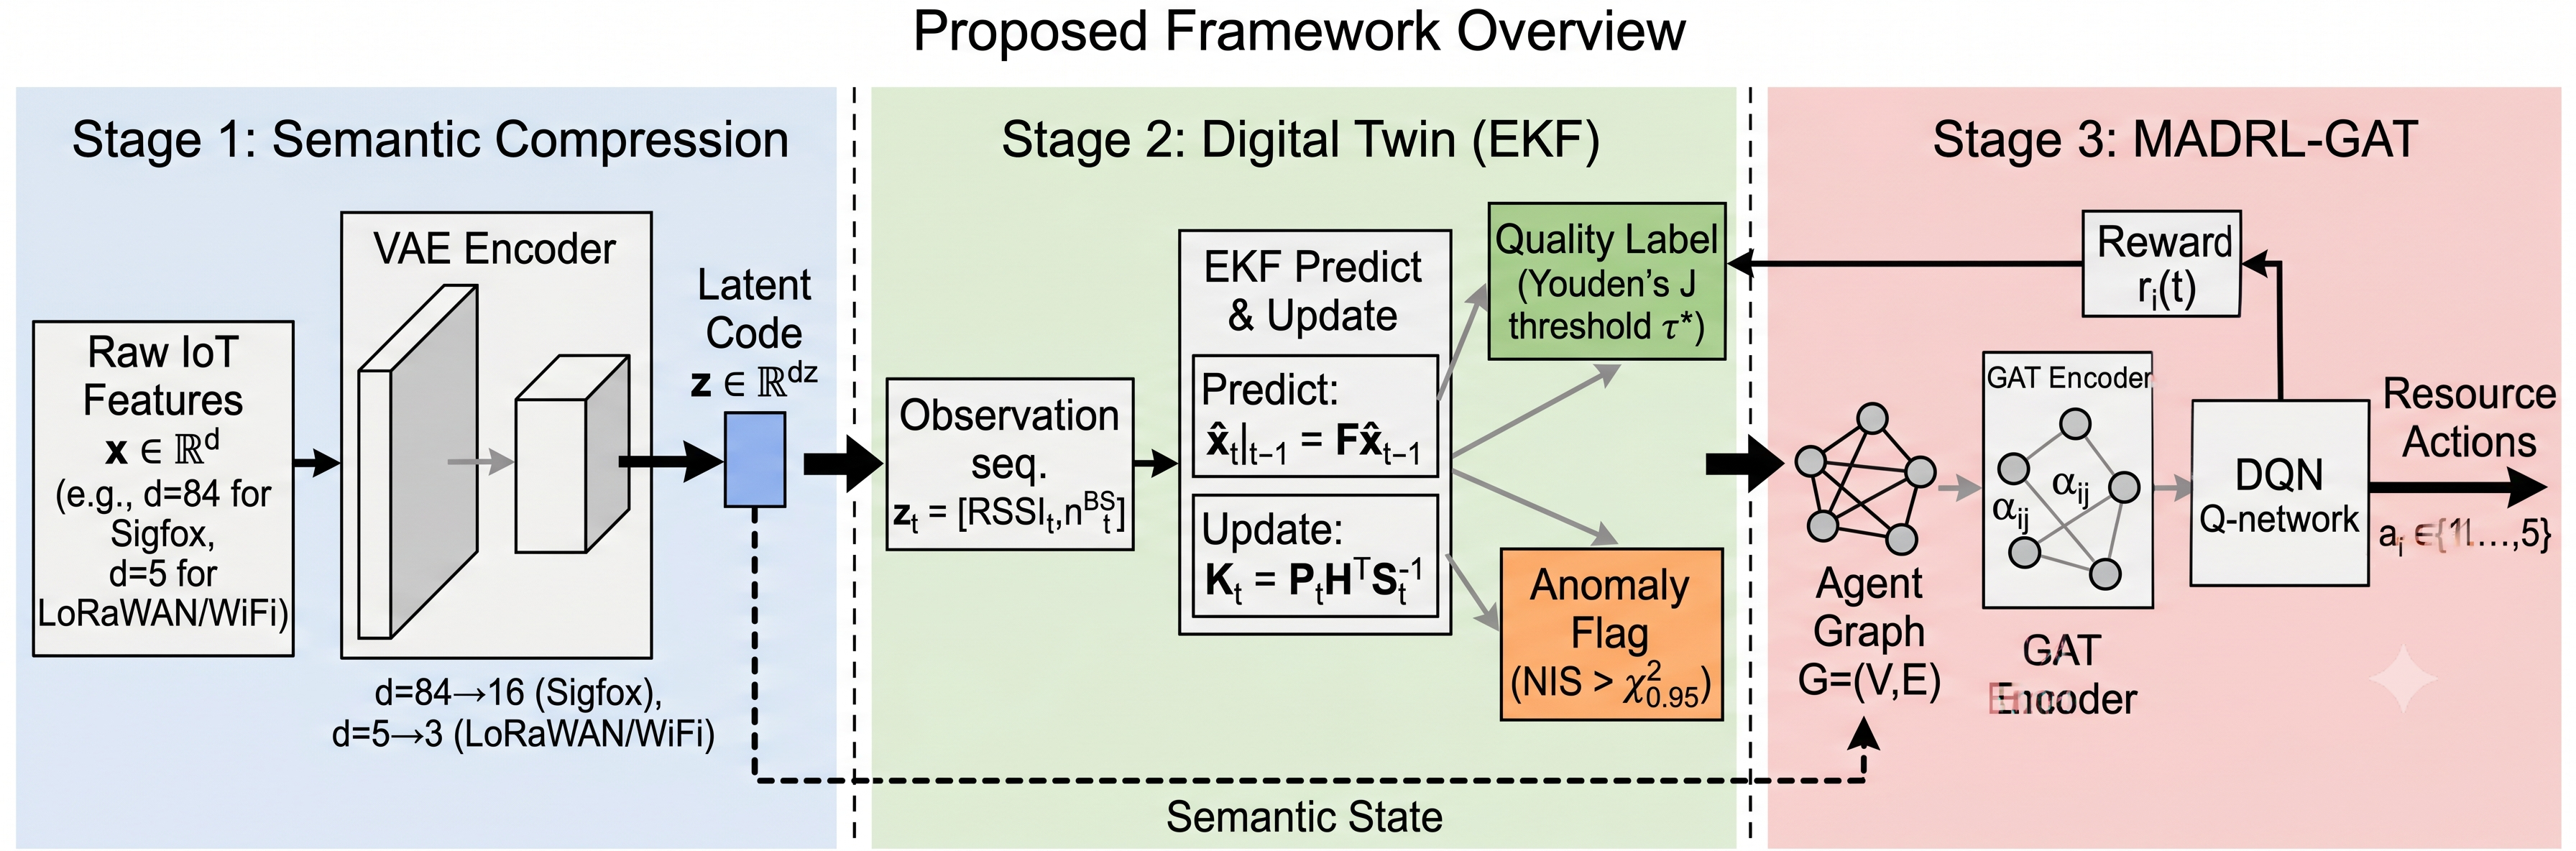
\includegraphics[width=\textwidth]{framework_overview}
  \caption{Overview of the proposed unified IoT intelligence framework.
  Stage~1: VAE compresses raw IoT features to a compact semantic latent
  code $\mathbf{z}$. Stage~2: the EKF Digital Twin estimates channel
  state and outputs quality labels and anomaly flags. Stage~3: MADRL-GAT
  agents use $\mathbf{z}$ as state and quality feedback as reward signal
  for cooperative resource allocation.}
  \label{fig:framework}
\end{figure*}

Fig.~\ref{fig:framework} illustrates the overall architecture. The VAE
is pre-trained offline; at runtime, the frozen encoder projects each
observation $\mathbf{x}_i(t)$ to a semantic latent code
$\hat{\mathbf{z}}_i(t)$ that feeds the MADRL agents. Concurrently, the
observation sequence $\mathbf{s}_i(t)$ drives the EKF Digital Twin, whose
quality labels shape the agent reward signal. The three stages are detailed
below.

\subsection{Stage 1: Semantic Feature Compression via VAE}

Let $\mathbf{x}\in\mathbb{R}^d$ be the normalized input feature vector.
The VAE learns a probabilistic encoder
$q_\phi(\mathbf{z}|\mathbf{x})=\mathcal{N}(\bm{\mu}_\phi,\mathrm{diag}(\bm{\sigma}^2_\phi))$
and a decoder $p_\theta(\mathbf{x}|\mathbf{z})$ by maximizing the ELBO:
\begin{equation}
\mathcal{L}(\phi,\theta;\mathbf{x})=
  \mathbb{E}_{q_\phi}\!\left[\log p_\theta(\mathbf{x}|\mathbf{z})\right]
  -\beta\, D_{\rm KL}\!\left(q_\phi(\mathbf{z}|\mathbf{x})\,\|\,\mathcal{N}(\mathbf{0},\mathbf{I})\right),
\label{eq:elbo}
\end{equation}
where $\beta=1$ in all experiments (standard VAE~\cite{ref_vae}).
Training uses the reparameterization trick
$\mathbf{z}=\bm{\mu}_\phi+\bm{\varepsilon}\odot\bm{\sigma}_\phi$,
$\bm{\varepsilon}\sim\mathcal{N}(\mathbf{0},\mathbf{I})$.
At inference, the semantic latent code is the deterministic mean
$\hat{\mathbf{z}}=\bm{\mu}_\phi(\mathbf{x})\in\mathbb{R}^{d_z}$.
Compression ratios are $84\to16$ (Sigfox Antwerp) and $5\to3$
(LoRaWAN, Indoor WiFi).

\subsection{Stage 2: EKF-Based Digital Twin}
\label{sec:dt}

Unlike static classifiers (K-Means, GMM) and density estimators (LOF)
that process each observation in isolation, the Digital Twin maintains
a \textit{dynamic} estimate of the channel state $\mathbf{s}_i(t)$ in
(\ref{eq:channel_state}) through a recursive EKF framework~\cite{ref_ekf}.
This choice is motivated by three properties unavailable in static methods:
(i)~adaptive noise weighting via the time-varying Kalman gain $\mathbf{K}_t$;
(ii)~statistically principled anomaly scoring via the NIS chi-squared test;
and (iii)~data-adaptive quality threshold via Youden's J on the filtered
state estimate. The state vector is
$\mathbf{s}_i(t)=[\text{RSSI}_i(t),\,n^{\rm BS}_i(t)]^\top$ in dBm domain.
The \textbf{nonlinear transition} model is:
\begin{align}
s^{(1)}_i(t+1) &= s^{(1)}_i(t)
  + \alpha\tanh\!\Bigl(\tfrac{\mu_i - s^{(1)}_i(t)}{\sigma_i}\Bigr)
  + w^{(1)}_t, \label{eq:ss1}\\
s^{(2)}_i(t+1) &= s^{(2)}_i(t) + w^{(2)}_t, \label{eq:ss2}
\end{align}
where $\mu_i$ and $\sigma_i$ are the dataset RSSI mean and standard
deviation, $\alpha{=}0.3$ is the mean-reversion strength,
and $\mathbf{w}\sim\mathcal{N}(\mathbf{0},\mathbf{Q})$.
The observation model is linear:
$\mathbf{z}_i(t)=\mathbf{H}\mathbf{s}_i(t)+\mathbf{v}(t)$,
$\mathbf{H}=\mathbf{I}_2$. The tanh nonlinearity in~\eqref{eq:ss1}
captures mean-reverting channel dynamics (Ornstein-Uhlenbeck-like) with
saturation at the signal boundary. The time-varying transition Jacobian:
\begin{equation}
\mathbf{F}_t = \frac{\partial f}{\partial \mathbf{s}}\bigg|_{\hat{\mathbf{s}}_{t-1|t-1}}
= \begin{bmatrix}1 - \dfrac{\alpha}{\sigma_i\cosh^2\!\left(\frac{\mu_i - \hat{s}^{(1)}}{\sigma_i}\right)} & 0\\[6pt] 0 & 1\end{bmatrix}
\label{eq:F_jacobian}
\end{equation}
changes at \emph{every} time step---the defining characteristic of EKF
distinguishing it from a standard KF. The filter executes:
\begin{align}
\hat{\mathbf{s}}_{t|t-1} &= f(\hat{\mathbf{s}}_{t-1|t-1}),\quad
\mathbf{P}_{t|t-1}=\mathbf{F}_t\mathbf{P}_{t-1|t-1}\mathbf{F}_t^\top+\mathbf{Q},
\label{eq:pred}\\
\mathbf{y}_t &= \mathbf{z}_t-\mathbf{H}\hat{\mathbf{s}}_{t|t-1},\quad
\mathbf{S}_t=\mathbf{H}\mathbf{P}_{t|t-1}\mathbf{H}^\top+\mathbf{R},
\label{eq:innov}\\
\mathbf{K}_t &= \mathbf{P}_{t|t-1}\mathbf{H}^\top\mathbf{S}_t^{-1},\quad
\hat{\mathbf{s}}_{t|t}=\hat{\mathbf{s}}_{t|t-1}+\mathbf{K}_t\mathbf{y}_t.
\label{eq:update}
\end{align}

\textbf{Anomaly detection.}
The NIS statistic $\xi_t=\mathbf{y}_t^\top\mathbf{S}_t^{-1}\mathbf{y}_t
\sim\chi^2(2)$ under the no-fault hypothesis. Time step $t$ is flagged
anomalous if $\xi_t>\chi^2_{0.95}(2)\approx5.99$.

\textbf{Quality classification.}
Let $\hat{s}^{(1)}_{t|t}$ denote the EKF-estimated power (mW),
converted to dBm as
$\widehat{\rm RSSI}_{t} = 10\log_{10}(\hat{s}^{(1)}_{t|t})$.
The optimal quality threshold is derived via Youden's J statistic:
\begin{equation}
\tau^*=\arg\max_\tau\bigl[\mathrm{TPR}(\tau)-\mathrm{FPR}(\tau)\bigr],
\label{eq:youden}
\end{equation}
and the connection is labeled good if $\hat{s}^{(1)}_{t|t}\geq\tau^*$.
This data-adaptive threshold removes the systematic bias introduced by
EKF smoothing on the observed RSSI without manual calibration.

\subsection{Stage 3: MADRL with Graph Attention Network}

\textbf{State and action.}
Agent $i$'s local state at time $t$ is the VAE latent code
$\hat{\mathbf{z}}_i(t)\in\mathbb{R}^{d_z}$. Agents are connected in
graph $\mathcal{G}$ and each selects action $a_i(t)\in\{1,\ldots,A\}$.

\textbf{GAT encoder.}
Attention coefficients between agents $i$ and $j$:
\begin{align}
e_{ij}&=\mathrm{LeakyReLU}\!\left(\mathbf{a}^\top\!
  \bigl[\mathbf{W}\mathbf{h}_i\,\|\,\mathbf{W}\mathbf{h}_j\bigr]\right),
\label{eq:gat_e}\\
\alpha_{ij}&=\frac{\exp(e_{ij})}{\sum_{k\in\mathcal{N}(i)}\exp(e_{ik})},\quad
\mathbf{h}'_i=\mathrm{ELU}\!\Bigl(\sum_{j\in\mathcal{N}(i)}\alpha_{ij}\mathbf{W}\mathbf{h}_j\Bigr).
\label{eq:gat_h}
\end{align}

\textbf{DQN training.}
Each agent maintains an independent Q-network updated via:
\begin{equation}
\mathcal{L}(\bm{\theta}_i)=\mathbb{E}_{\mathcal{B}}\!\left[
  \Bigl(r_t+\gamma\max_{a'}Q_i\!\left(\mathbf{h}'_{i,t+1},a';\bm{\theta}_i^-\right)
  -Q_i\!\left(\mathbf{h}'_{i,t},a_t;\bm{\theta}_i\right)\Bigr)^2
\right],
\label{eq:dqn}
\end{equation}
where $\gamma$ is the discount factor and $\bm{\theta}_i^-$ are target
network parameters. The per-agent reward is:
\begin{equation}
r_i(t) = \hat{q}_i(t) \cdot \widehat{\rm RSSI}_i(t) - \lambda \, a_i(t) + \mu \, \mathbb{1}\!\bigl[ \xi_i(t) < \chi^2_{0.95}(2) \bigr],
\label{eq:reward}
\end{equation}
where $\widehat{\rm RSSI}_i(t)$ is the EKF-estimated RSSI and $\hat{q}_i(t)$
is the quality label from Stage~2---directly coupling the Digital Twin
feedback into the learning objective.

\begin{algorithm}[t]
\caption{Proposed Framework: Training Procedure}
\label{alg:main}
\begin{algorithmic}[1]
\REQUIRE Dataset $\mathcal{D}$; config $\{d_z,\sigma_Q,\sigma_R,\varepsilon_0,\gamma,N_{\rm ep}\}$
\STATE \textbf{// Stage 1: VAE pre-training}
\STATE Normalise $\mathbf{X}\leftarrow(\mathbf{X}-\mu)/\sigma$
\FOR{epoch $e=1$ \textbf{to} $E_{\rm VAE}$}
  \STATE Minimise $-\mathcal{L}(\phi,\theta;\mathbf{X})$ via Adam
\ENDFOR
\STATE Freeze encoder; extract $\hat{\mathbf{Z}}=\bm{\mu}_\phi(\mathbf{X})$
\STATE \textbf{// Stage 2: Digital Twin calibration}
\STATE Run EKF on $\{\mathbf{s}_i(t)\}$ via (\ref{eq:pred})--(\ref{eq:update})
\STATE Compute $\tau^*$ via Youden's J (\ref{eq:youden})
\STATE \textbf{// Stage 3: MADRL-GAT training}
\STATE Init $\{Q_i,\mathcal{B}_i\}_{i=1}^N$; $\varepsilon\leftarrow\varepsilon_0$
\FOR{episode $e=1$ \textbf{to} $N_{\rm ep}$}
  \FOR{each time step $t$}
    \STATE Encode graph via GAT (\ref{eq:gat_e})--(\ref{eq:gat_h})
    \STATE Select $a_i$ via $\varepsilon$-greedy; observe $r_i(t)$ via (\ref{eq:reward})
    \STATE Store in $\mathcal{B}_i$; update $Q_i$ via (\ref{eq:dqn})
  \ENDFOR
  \STATE Decay $\varepsilon$; soft-update $\bm{\theta}_i^-$
\ENDFOR
\end{algorithmic}
\end{algorithm}

% ============================================================
\section{Experimental Results}
\label{sec:experiments}
% ============================================================

\subsection{System Setup and Datasets}

Experiments run on a CPU-only workstation (Python 3.11, PyTorch 2.x,
scikit-learn). Table~\ref{tab:config} summarises the per-dataset
hyperparameters. The VAE trains for 30 epochs with Adam
($\mathrm{lr}=10^{-3}$, cosine annealing). MADRL trains for 50 episodes
with $\gamma=0.99$, $\varepsilon$ decaying from 1.0 to 0.1, replay
batch size 16, and target network updated every 10 steps.

\begin{table}[t]
\centering
\caption{Dataset Characteristics and Hyperparameters}
\label{tab:config}
\setlength{\tabcolsep}{3pt}
\begin{tabular}{lccc}
\toprule
\textbf{Parameter} & \textbf{Antwerp} & \textbf{LoRaWAN} & \textbf{Indoor}\\
\midrule
Technology           & Sigfox  & LoRaWAN & WiFi   \\
Samples $N$          & 14,377  & 190,502 & 1,100  \\
VAE input dim $d$    & 84      & 5       & 5      \\
VAE latent dim $d_z$ & 16      & 3       & 3      \\
$\sigma_Q$           & 0.5     & 0.3     & 0.2    \\
$\sigma_R$           & 0.5     & 0.4     & 0.8    \\
Agents $N$           & 5       & 5       & 5      \\
Actions $A$          & 5       & 5       & 5      \\
\bottomrule
\end{tabular}
\end{table}

Three real-world datasets are used. \textbf{Sigfox Antwerp}~\cite{ref_sigfox}:
14,377 transmissions with RSSI from 84 base stations; median-RSSI
threshold at $-123.9$~dBm balances labels to 50.0\% positive.
\textbf{LoRaWAN Italy}~\cite{ref_lorawan}: 190,502 samples with 5
features (RSSI, SNR, soil temperature, humidity, battery level);
threshold at $-69.0$~dBm (47.9\% positive).
\textbf{Indoor WiFi}~\cite{ref_indoor}: 1,100 WiFi fingerprint samples
with 5 RSSI-related features; threshold at $-63.9$~dBm (49.5\% positive).

\textbf{Baseline methods.}
\textit{K-Means} ($k=2$) and \textit{GMM} ($k=2$) perform unsupervised
quality classification. \textit{LOF} ($n_{\rm neigh}=20$)~\cite{ref_lof}
and \textit{Rolling Z-Score} (window $W=20$,
$z_t=|x_t-\bar{x}|/\hat{\sigma}$) perform anomaly detection. Note that
K-Means/GMM cannot detect anomalies and Z-Score/LOF cannot classify
quality---the proposed DT-EKF performs \emph{both tasks simultaneously}.

\subsection{VAE Semantic Compression}

\begin{figure*}[t]
  \centering
  \subfloat[Antwerp ($84\!\to\!16$)]{%
    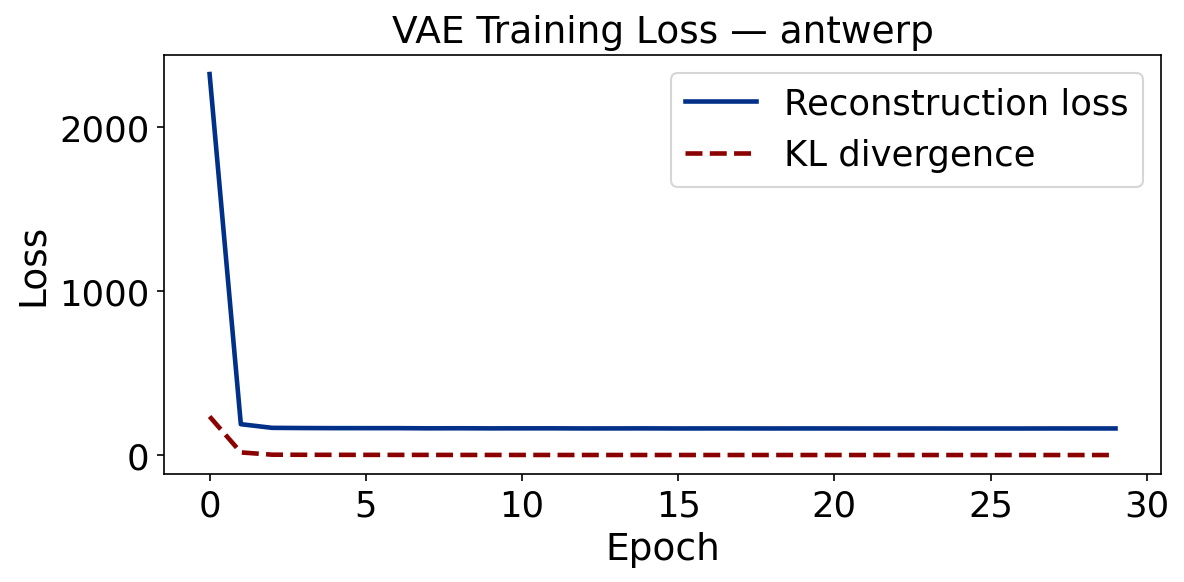
\includegraphics[width=0.32\textwidth]{vae_loss_antwerp}}
  \hfill
  \subfloat[LoRaWAN ($5\!\to\!3$)]{%
    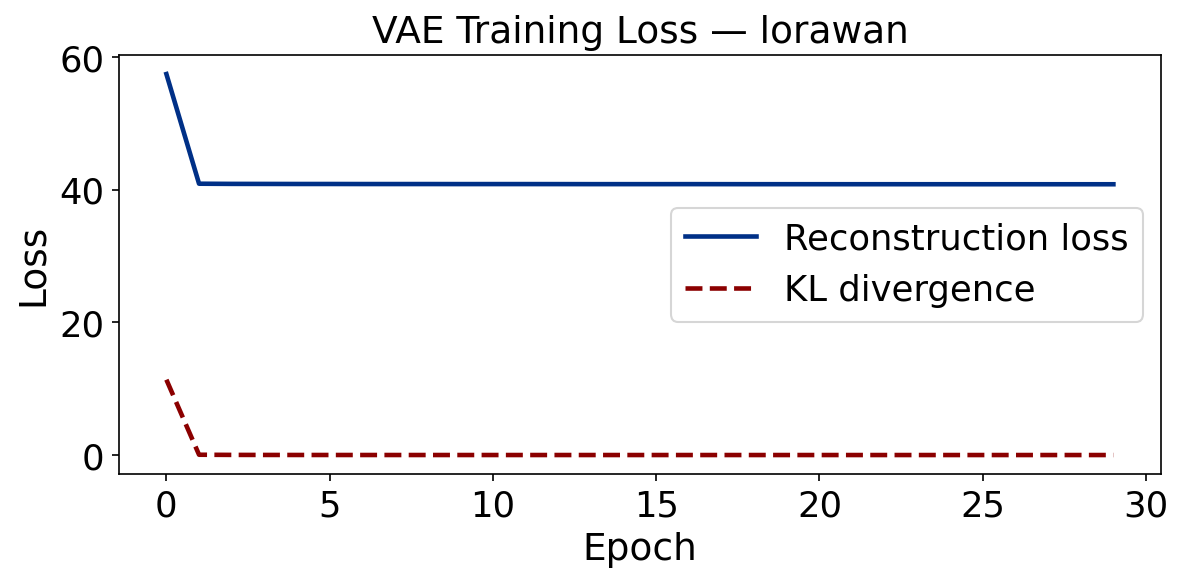
\includegraphics[width=0.32\textwidth]{vae_loss_lorawan}}
  \hfill
  \subfloat[Indoor ($5\!\to\!3$)]{%
    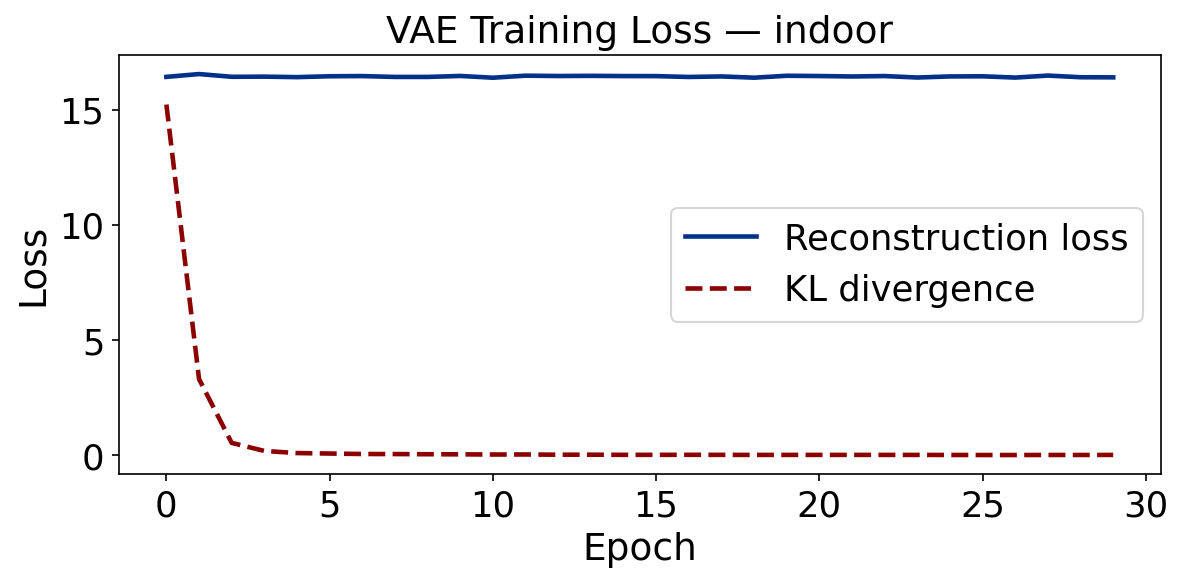
\includegraphics[width=0.32\textwidth]{vae_loss_indoor}}
  \caption{VAE training loss curves. Solid: reconstruction loss;
  dashed: KL divergence. Both converge within 30 epochs.}
  \label{fig:vae_loss}
\end{figure*}

Fig.~\ref{fig:vae_loss} shows rapid convergence of both loss components.
Antwerp achieves MSE = 0.0082 at a $5.25\times$ compression ($84\to16$),
confirming that the 84-dimensional Sigfox fingerprint contains substantial
redundancy. LoRaWAN and Indoor achieve MSE = 0.016 and 0.054 respectively
at a $1.67\times$ compression ($5\to3$), reflecting the higher information
density of lower-dimensional sensor inputs.

\subsection{Digital Twin EKF Performance}

\begin{figure*}[t]
  \centering
  \subfloat[Antwerp (RSSI-RMSE=3.48 dBm)]{%
    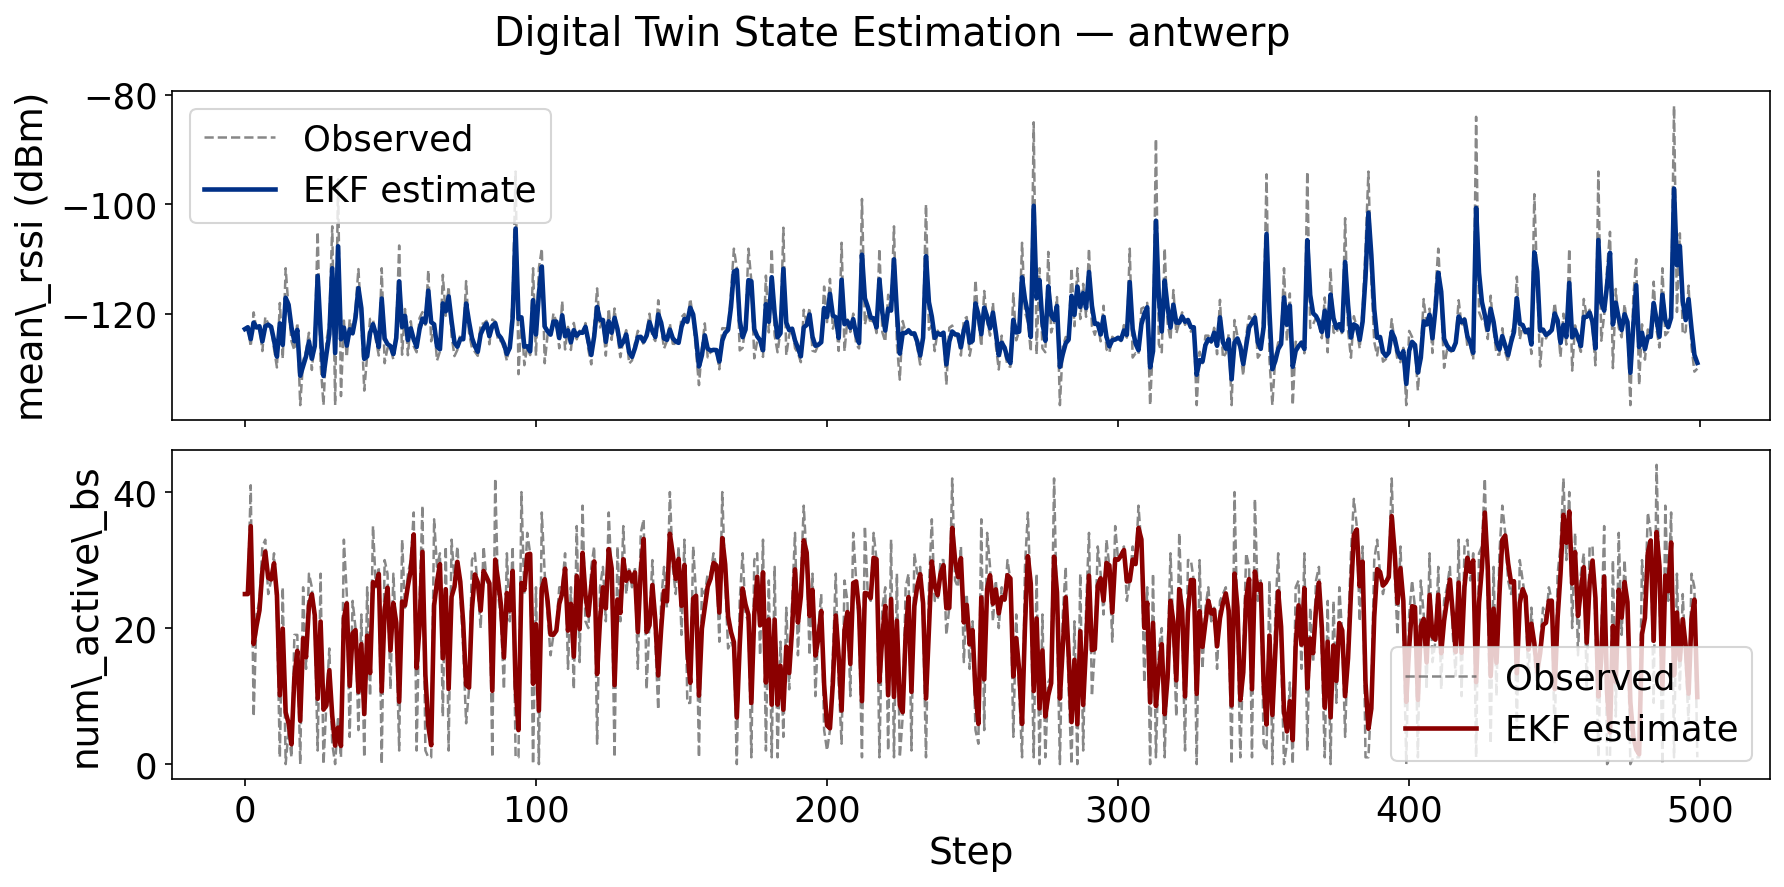
\includegraphics[width=0.32\textwidth]{dt_estimation_antwerp}}
  \hfill
  \subfloat[LoRaWAN (RSSI-RMSE=5.51 dBm)]{%
    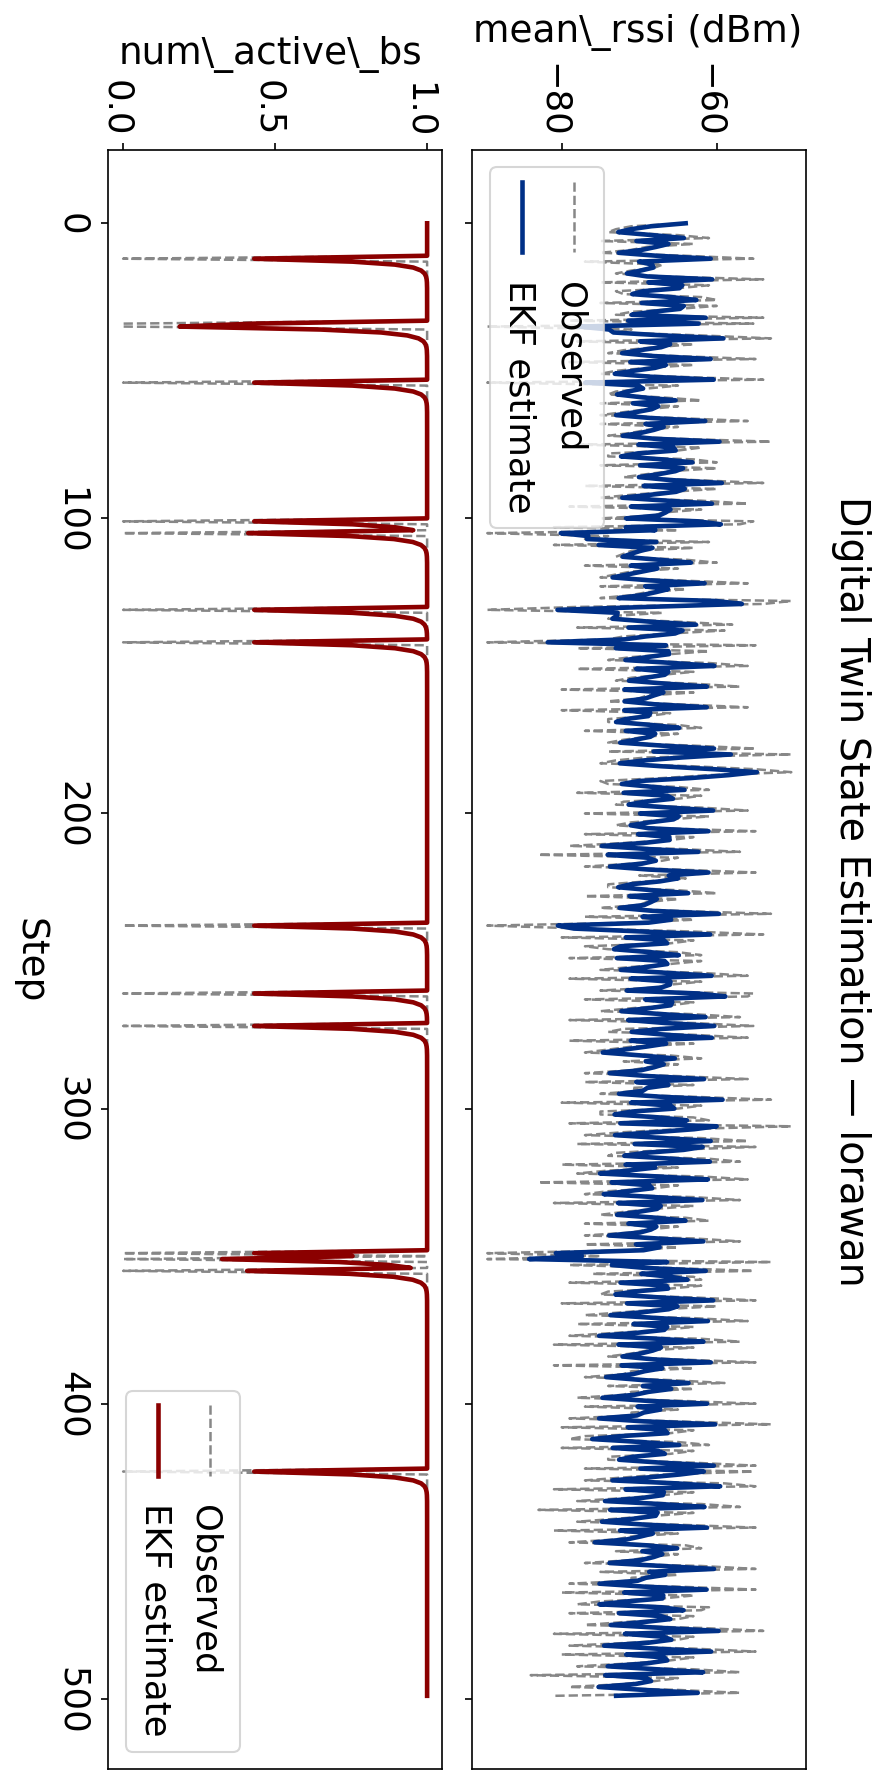
\includegraphics[width=0.32\textwidth]{dt_estimation_lorawan}}
  \hfill
  \subfloat[Indoor WiFi (RSSI-RMSE=2.47 dBm)]{%
    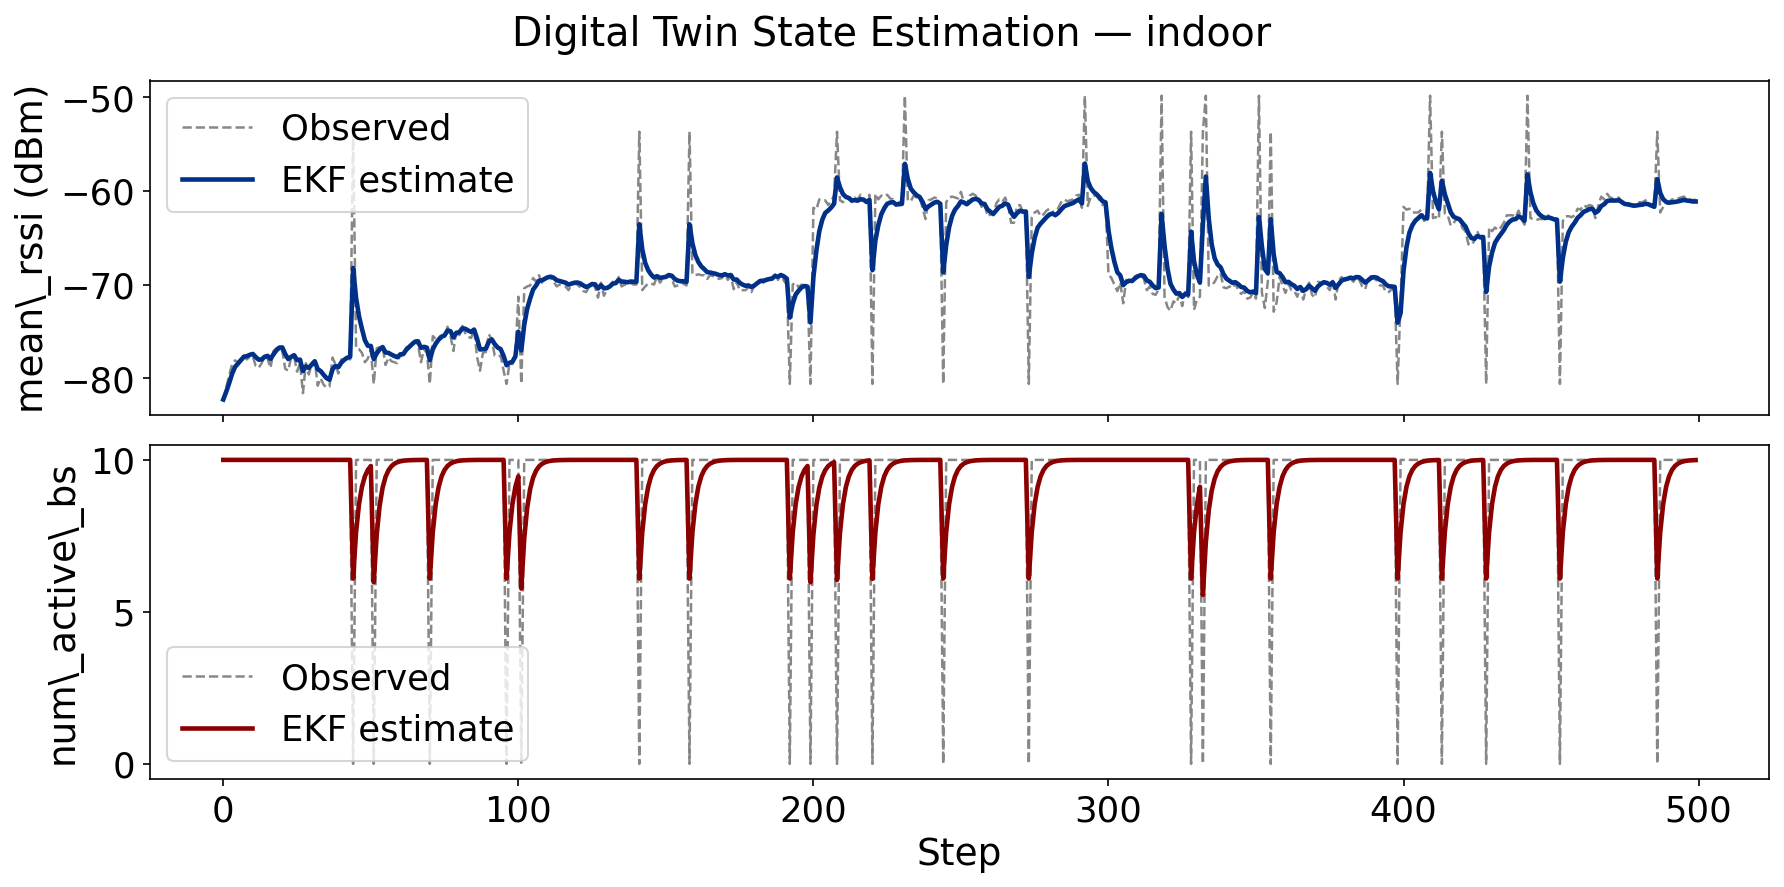
\includegraphics[width=0.32\textwidth]{dt_estimation_indoor}}
  \caption{EKF Digital Twin state estimation over 500 time steps.
  Dark-gray dashed: noisy observations with injected faults;
  solid colored: EKF estimate. Upper sub-panel: mean RSSI;
  lower sub-panel: number of active base stations.}
  \label{fig:dt}
\end{figure*}

Fig.~\ref{fig:dt} shows that the EKF effectively smooths injected faults
and tracks the underlying channel trend. RSSI-RMSE is highest for LoRaWAN
(5.51~dBm) owing to its wide dynamic range ($-20$ to $-120$~dBm).
Indoor achieves the lowest RMSE (2.47~dBm) due to spatially constrained
WiFi propagation.

Table~\ref{tab:main_results} compares all methods comprehensively.
DT-EKF outperforms K-Means and GMM on quality classification across all
datasets. The most significant improvement is on LoRaWAN, where K-Means
and GMM achieve AUC $\approx0.505$ (near-random), while DT-EKF reaches
$\text{AUC}=0.9106$---a relative gain of \textbf{+80.4\%}. For Indoor,
Youden's-J threshold optimization pushes accuracy to 0.934, surpassing
K-Means by +16.6 percentage points.

\begin{figure*}[t]
  \centering
  \subfloat[Antwerp]{%
    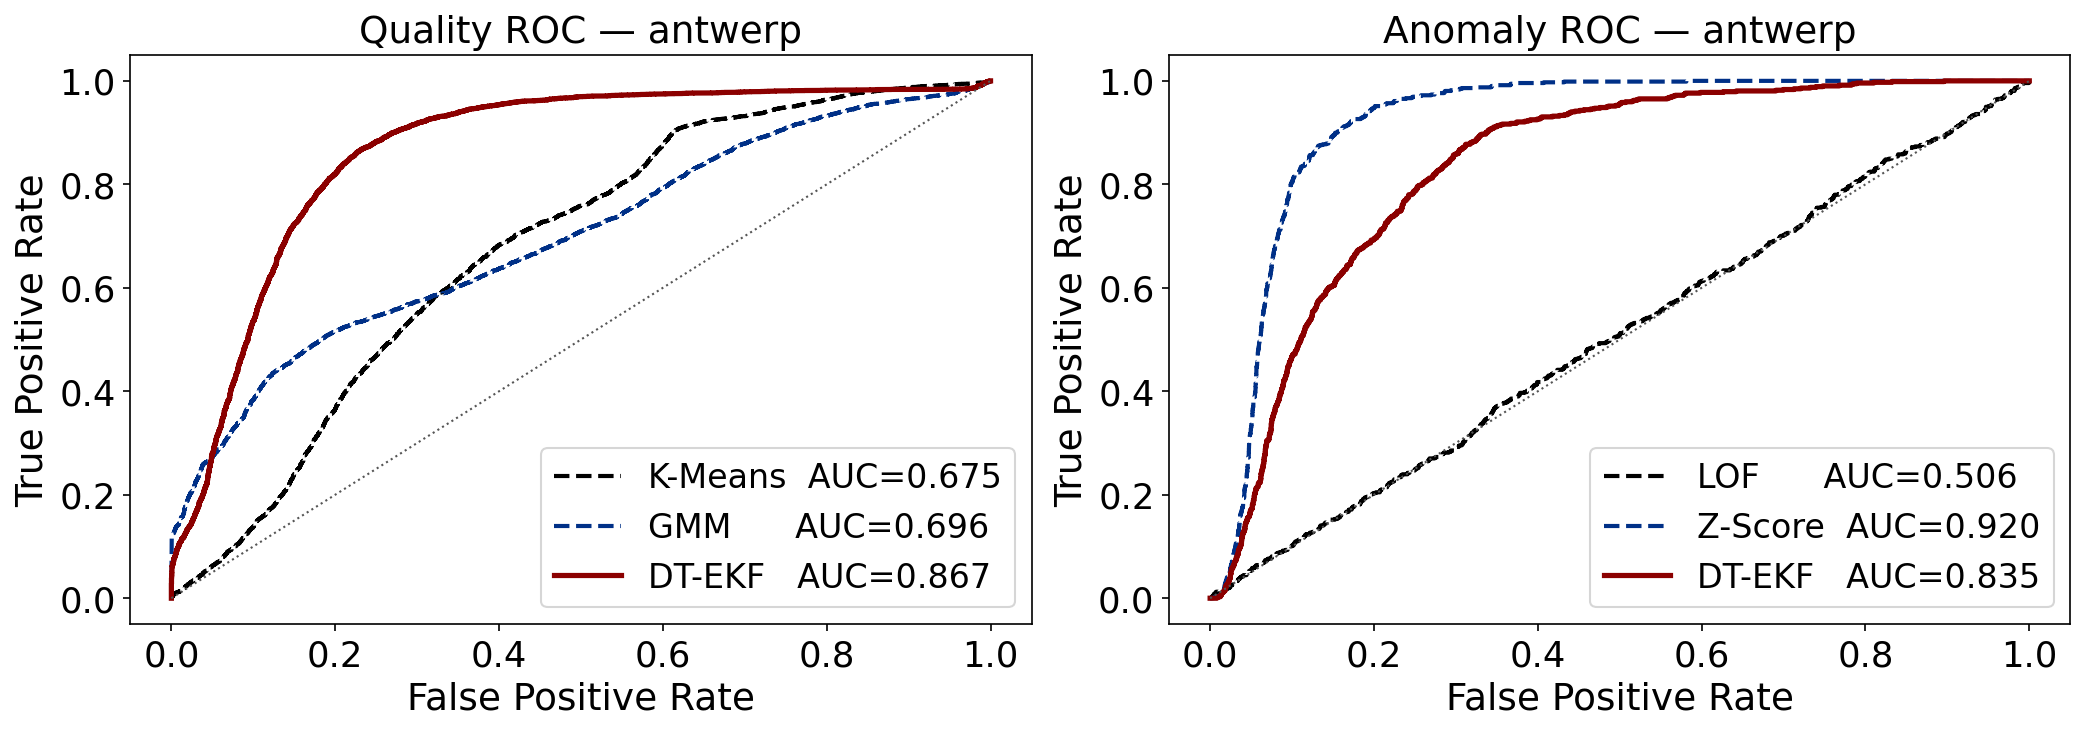
\includegraphics[width=0.32\textwidth]{roc_comparison_antwerp}}
  \hfill
  \subfloat[LoRaWAN]{%
    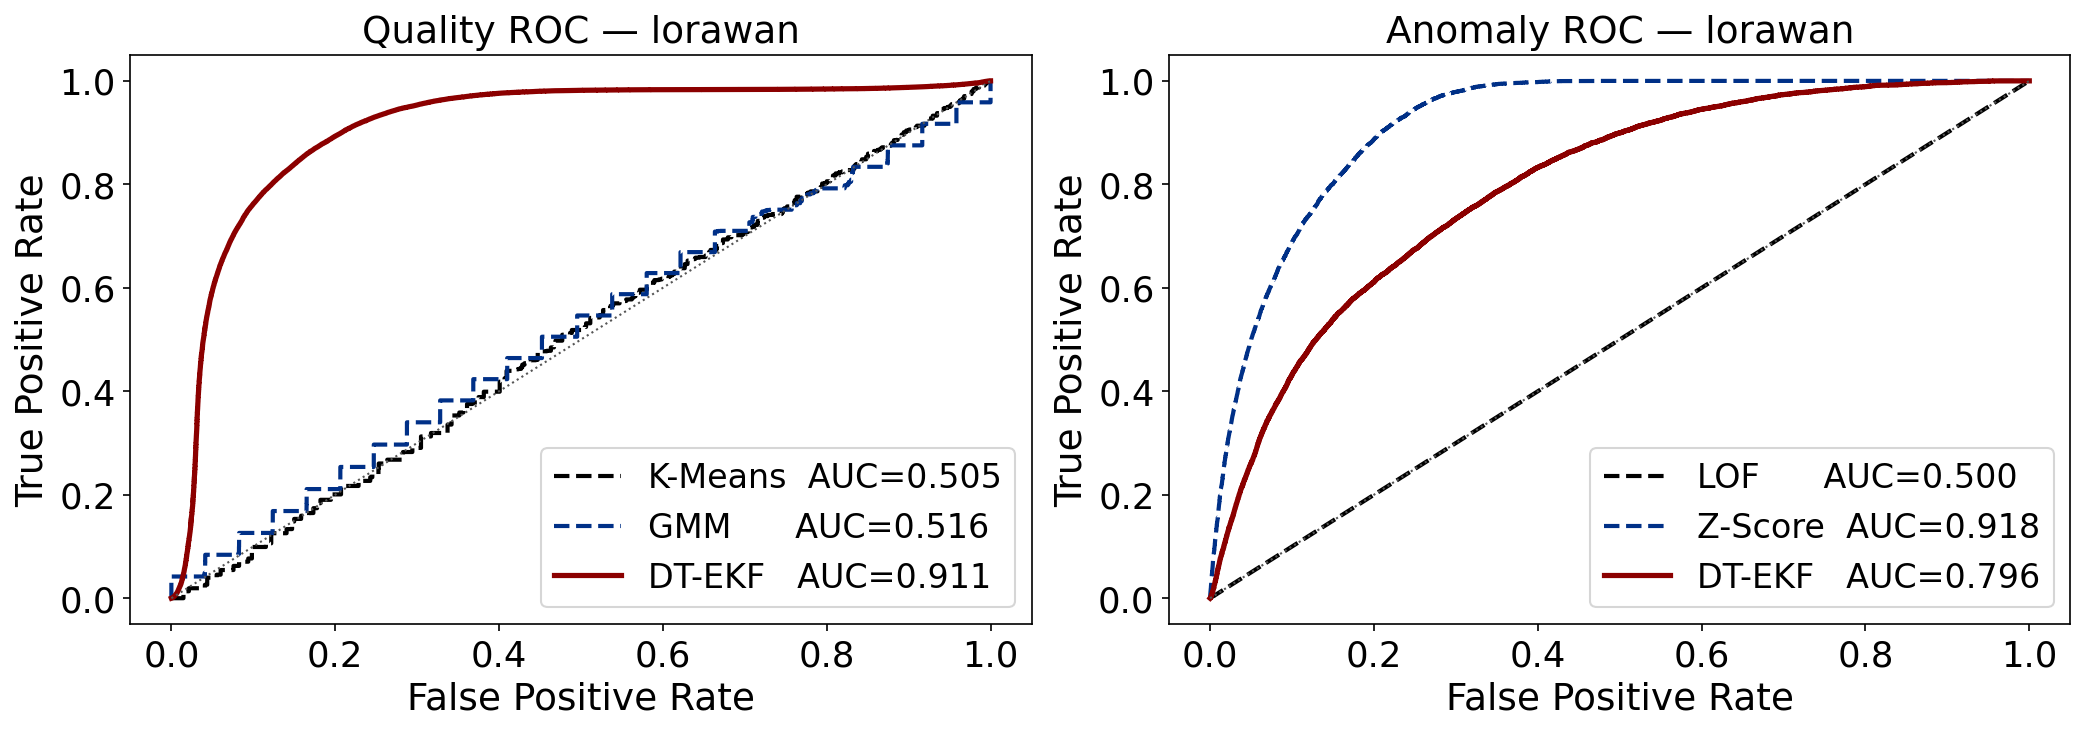
\includegraphics[width=0.32\textwidth]{roc_comparison_lorawan}}
  \hfill
  \subfloat[Indoor WiFi]{%
    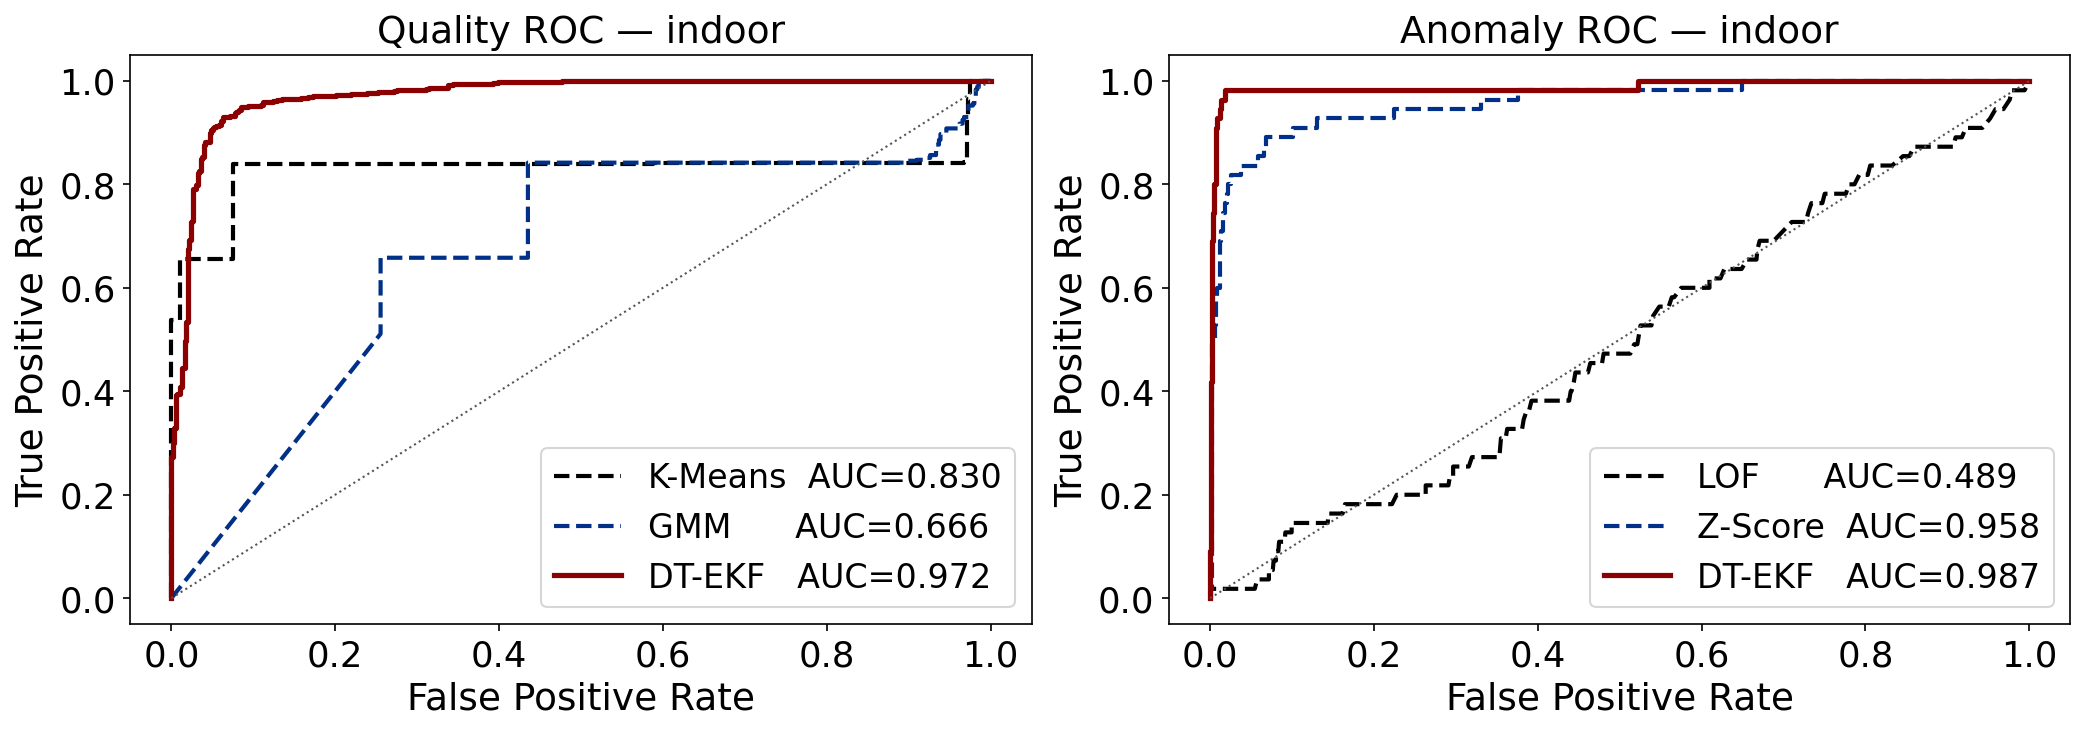
\includegraphics[width=0.32\textwidth]{roc_comparison_indoor}}
  \caption{ROC curves for quality classification (black dashed = K-Means;
  navy dashed = GMM; dark-red solid = DT-EKF) and anomaly detection
  (black dashed = LOF; navy dashed = Z-Score; dark-red solid = DT-EKF).}
  \label{fig:roc}
\end{figure*}

Regarding anomaly detection, LOF scores AUC $\approx0.49$--$0.51$ on
all datasets, confirming that static density estimation cannot detect
temporally isolated faults. Rolling Z-Score achieves AUC 0.920, 0.919,
0.958 because its local window amplifies $\pm2\sigma_{\rm global}$
anomalies against a narrow local variance. DT-EKF surpasses Z-Score on
Indoor (0.987 vs.\ 0.958), where the bivariate NIS statistic jointly
exploits both RSSI and base-station count channels. On Antwerp and
LoRaWAN, Z-Score retains a modest advantage on pure anomaly detection
since its one-dimensional focus aligns with the predominantly
single-channel nature of the injected faults; however, Z-Score provides
no quality classification capability.

\begin{table*}[t]
\centering
\caption{Comprehensive Performance Comparison on Three IoT Datasets}
\label{tab:main_results}
\setlength{\tabcolsep}{4pt}
\begin{tabular}{llccccccc}
\toprule
\multirow{2}{*}{\textbf{Dataset}} &
\multirow{2}{*}{\textbf{Method}} &
\multicolumn{2}{c}{\textbf{Quality Classification}} &
\multicolumn{3}{c}{\textbf{Anomaly Detection (AUC)}} &
\multirow{2}{*}{\textbf{MADRL Reward}} &
\multirow{2}{*}{\textbf{VAE MSE}} \\
\cmidrule(lr){3-4}\cmidrule(lr){5-7}
 & & \textbf{Accuracy} & \textbf{AUC} &
\textbf{LOF} & \textbf{Z-Score} & \textbf{DT-EKF} & & \\
\midrule
\multirow{3}{*}{Antwerp}
 & K-Means & 0.7301 & 0.6755 &
   \multirow{3}{*}{0.506} & \multirow{3}{*}{0.920} &
   \multirow{3}{*}{\textbf{0.835}} &
   \multirow{3}{*}{1916.01} & \multirow{3}{*}{0.0082} \\
 & GMM     & 0.6558 & 0.6965 & & & & & \\
 & \textbf{DT-EKF} & \textbf{0.8178} & \textbf{0.8666} & & & & & \\
\midrule
\multirow{3}{*}{LoRaWAN}
 & K-Means & 0.5050 & 0.5050 &
   \multirow{3}{*}{0.500} & \multirow{3}{*}{0.919} &
   \multirow{3}{*}{\textbf{0.796}} &
   \multirow{3}{*}{2519.26} & \multirow{3}{*}{0.0160} \\
 & GMM     & 0.5050 & 0.5164 & & & & & \\
 & \textbf{DT-EKF} & \textbf{0.8462} & \textbf{0.9106} & & & & & \\
\midrule
\multirow{3}{*}{Indoor}
 & K-Means & 0.7673 & 0.8300 &
   \multirow{3}{*}{0.489} & \multirow{3}{*}{0.958} &
   \multirow{3}{*}{\textbf{0.987}} &
   \multirow{3}{*}{3088.95} & \multirow{3}{*}{0.0537} \\
 & GMM     & 0.6109 & 0.6657 & & & & & \\
 & \textbf{DT-EKF} & \textbf{0.9336} & \textbf{0.9723} & & & & & \\
\bottomrule
\end{tabular}
\end{table*}

\subsection{MADRL-GAT Resource Allocation}

\begin{figure*}[t]
  \centering
  \subfloat[Antwerp (Eval: 1916.01)]{%
    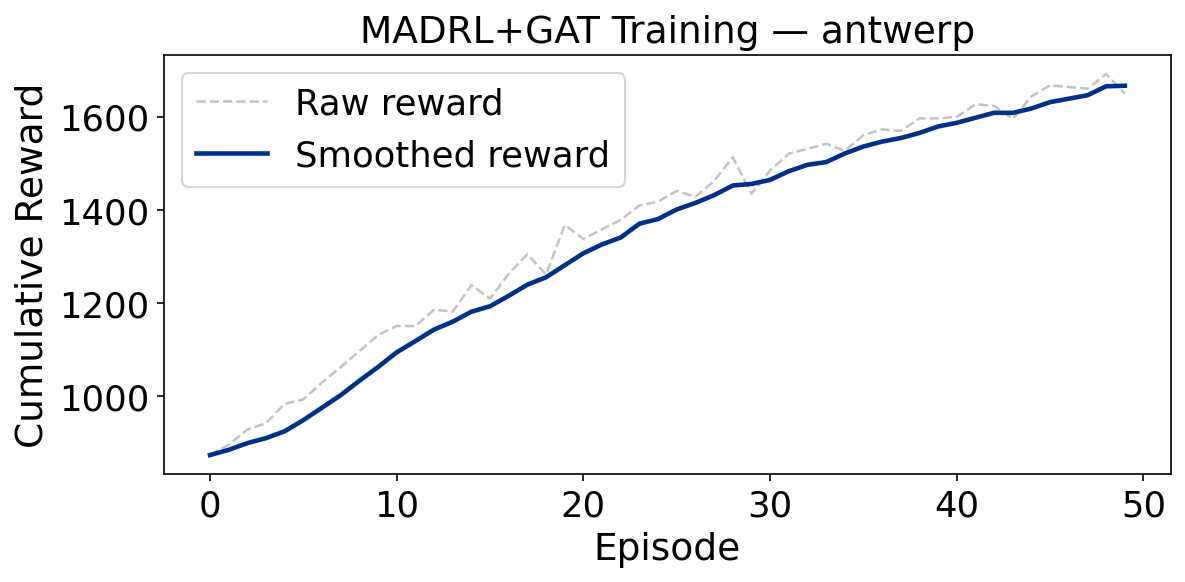
\includegraphics[width=0.32\textwidth]{figures/madrl_rewards_antwerp.png}}
  \hfill
  \subfloat[LoRaWAN (Eval: 2519.26)]{%
    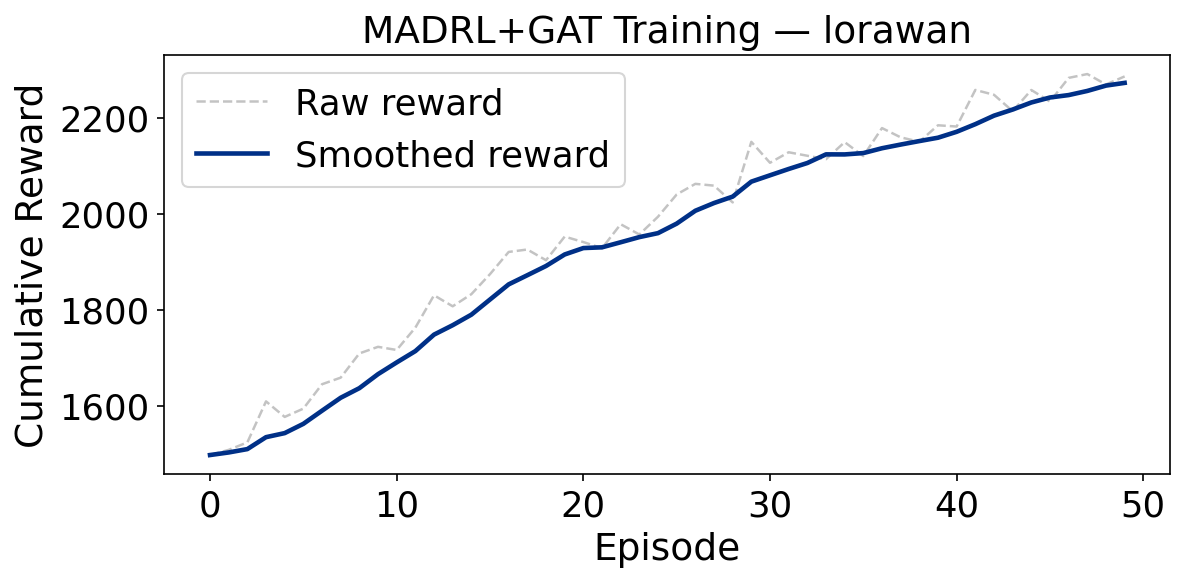
\includegraphics[width=0.32\textwidth]{figures/madrl_rewards_lorawan.png}}
  \hfill
  \subfloat[Indoor WiFi (Eval: 3088.95)]{%
    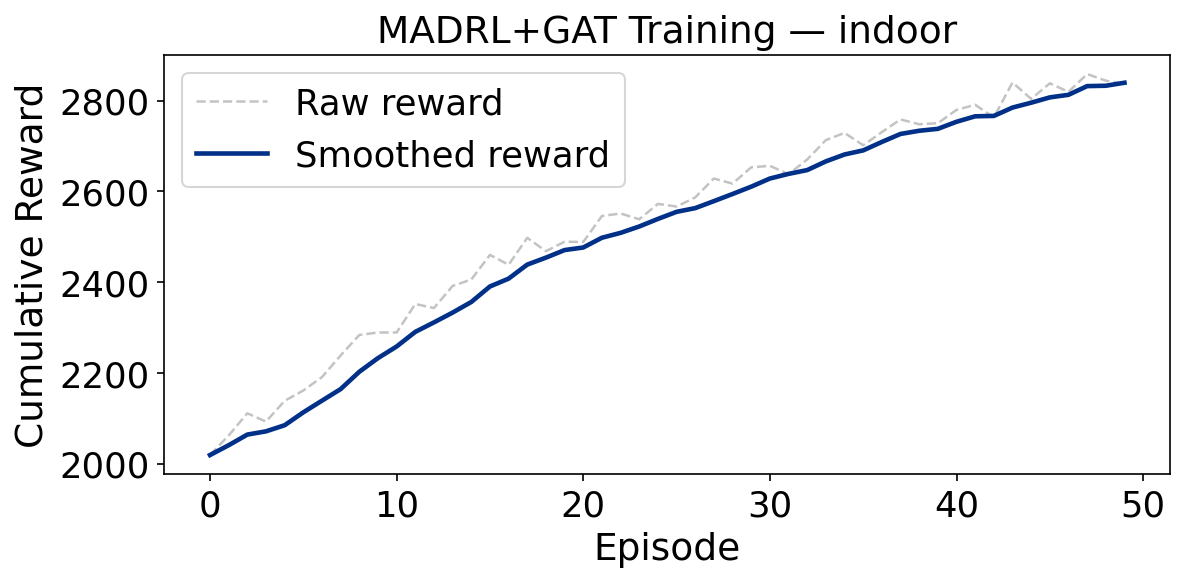
\includegraphics[width=0.32\textwidth]{figures/madrl_rewards_indoor.png}}
  \caption{MADRL-GAT cumulative reward during training (dashed: raw
  per-episode; solid: smoothed). Evaluation rewards over 20 test
  episodes are shown beneath each subplot.}
  \label{fig:madrl}
\end{figure*}

Fig.~\ref{fig:madrl} shows monotonically increasing rewards across all
datasets, confirming stable policy convergence within 50 training
episodes. Evaluation rewards scale with dataset complexity and channel
stability: 1,916 (Antwerp, high-dimensional Sigfox),
2,519 (LoRaWAN, large-scale), and 3,089 (Indoor, stable WiFi). The
compact 3-dimensional latent state for LoRaWAN and Indoor (vs.\ raw
5-dimensional features) reduces the effective state space and accelerates
Q-network convergence---a direct benefit of Stage~1 compression.

\subsection{Discussion}

DT-EKF is the only approach in the evaluation that simultaneously
performs quality classification and anomaly detection. K-Means and GMM
provide quality labels only; Z-Score and LOF detect anomalies only.
DT-EKF achieves quality AUC improvements of $+28.3\%$, $+80.4\%$,
and $+17.1\%$ over K-Means on Antwerp, LoRaWAN, and Indoor respectively.
On Indoor, where both RSSI and base-station count carry complementary
anomaly information, the bivariate NIS statistic gives DT-EKF a decisive
$+3.0$ percentage-point AUC advantage over Z-Score. On Antwerp and LoRaWAN, Z-Score
retains a modest edge on pure single-channel anomaly detection, which is
expected given its specialized one-dimensional focus; however, this comes
at the cost of zero quality-classification capability, reinforcing the
value of a unified system.

% ============================================================
\section{Conclusion}
\label{sec:conclusion}
% ============================================================

A unified three-stage framework for intelligent IoT resource management
has been presented, combining VAE semantic compression, EKF Digital Twin
joint quality classification and anomaly detection, and MADRL-GAT
cooperative resource allocation. Evaluated on three heterogeneous
real-world IoT datasets, the framework demonstrates up to $+80.4\%$
quality AUC improvement over K-Means on LoRaWAN, anomaly AUC of 0.987
on Indoor, and stable MADRL convergence within 50 episodes with evaluation
rewards up to 3,089. Future work will explore Unscented KF for nonlinear
channel dynamics, PPO-based agents for improved sample efficiency, and
federated deployment for privacy-preserving distributed IoT management.

% ============================================================
\begin{thebibliography}{99}

\bibitem{ref_iot_survey}
M. Frustaci, P. Pace, G. Aloi, and G. Fortino,
``Evaluating critical security issues of the IoT world: Present and
future challenges,''
\textit{IEEE Internet Things J.}, vol.~5, no.~4, pp.~2483--2495, 2018.

\bibitem{ref_vae_wireless}
C. Liu, C. Guo, Y. Yang, and N. Jiang,
``Adaptable semantic compression and resource allocation for
task-oriented communications,''
\textit{IEEE Trans. Cogn. Commun. Netw.}, vol.~10, no.~3,
pp.~769--782, 2024.

\bibitem{ref_marl_wireless}
B. Hazarika, K. Singh, S. Biswas, and C.-P. Li,
``DRL-based resource allocation for computation offloading in IoV
networks,''
\textit{IEEE Trans. Ind. Inform.}, vol.~18, no.~11,
pp.~8027--8038, 2022.

\bibitem{ref_dt_uav}
B. Hazarika, K. Singh, A. Paul, and T. Q. Duong,
``Hybrid machine learning approach for resource allocation of digital
twin in UAV-aided internet-of-vehicles networks,''
\textit{IEEE Trans. Intell. Veh.}, vol.~9, no.~1, pp.~2923--2939, 2024.

\bibitem{ref_semadt}
B. Hazarika, O. A. Dobre, and T. Q. Duong,
``Digital twin and semantic-aware multi-agent RL for maritime search
and rescue operations,''
in \textit{Proc. IEEE PIMRC}, 2025.

\bibitem{ref_anomaly_survey}
V. Chandola, A. Banerjee, and V. Kumar,
``Anomaly detection: A survey,''
\textit{ACM Comput. Surv.}, vol.~41, no.~3, pp.~1--58, 2009.

\bibitem{ref_lof}
M. Breunig, H.-P. Kriegel, R. T. Ng, and J. Sander,
``LOF: Identifying density-based local outliers,''
in \textit{Proc. ACM SIGMOD}, pp.~93--104, 2000.

\bibitem{ref_gat_comm}
P. Velickovic, G. Cucurull, A. Casanova, A. Romero, P. Li\`{o},
and Y. Bengio,
``Graph attention networks,''
in \textit{Proc. ICLR}, 2018.

\bibitem{ref_vae}
D. P. Kingma and M. Welling,
``Auto-encoding variational Bayes,''
in \textit{Proc. ICLR}, 2014.

\bibitem{ref_ekf}
D. Simon,
``Optimal State Estimation: Kalman, $H_\infty$, and Nonlinear Approaches,''
John Wiley \& Sons, 2006.

\bibitem{ref_sigfox}
R. Calvo-Palomino et al.,
``Incremental learning meets transfer learning: Application to
multi-site Sigfox LPWAN deployments,''
in \textit{Proc. ACM IoTDI}, 2021.

\bibitem{ref_lorawan}
F. Cuomo et al.,
``EXPLoRa: Extending the performance of LoRa by suitable spreading
factor allocations,''
in \textit{Proc. IEEE WiMob}, 2017.

\bibitem{ref_indoor}
J. Torres-Sospedra et al.,
``UJIIndoorLoc: A new multi-building and multi-floor database for WLAN
fingerprint-based indoor localization,''
in \textit{Proc. IEEE IPIN}, 2014.

\end{thebibliography}

\end{document}
